\documentclass[reqno]{amsart}

\usepackage{External/takodachi}
\usepackage{slashed}

% To show labels in the margin:
\usepackage[notref, notcite]{showkeys}
\usepackage{xcolor}

% stupid amsart shows * headers in ToC
\DeclareRobustCommand{\SkipTocEntry}[5]{}

\newcommand{\arctanh}{\operatorname{arctanh}}
\renewcommand{\d}{\mathrm{d}}
\newcommand{\sfED}{\mathsf{ED}}
\newcommand{\sfS}{\mathsf S}
\newcommand{\sfN}{\mathsf N}

\title
{
	Global well-posedness and scattering for the energy-critical defocusing non-linear wave equation
} 
\author{Jason Zhao}
\date{\today}


\begin{document}
\maketitle

\begin{abstract}
	We give a new proof of the threshold theorem for the energy-critical non-linear wave equation using the energy dispersion + bubbling method of Sterbenz and Tataru.
\end{abstract}

\tableofcontents

\section{Introduction}
Before getting into any multi-linear algebra, it is important to get a grasp of coordinates in linear algebra and how these coordinates respond to change of bases. Let $V$ be an $n$-dimensional real vector space, and denote $V^*$ its dual space. Given a basis $\{e_i\}_i \subseteq V$, there exists a dual basis $\{\epsilon^j\}_j \subseteq V^*$ satisfying 
	\[ \langle e_i, \epsilon^j \rangle = \delta^j_i. \]
Choose another basis $\{\widetilde e_i\}_i \subseteq V$ and denote its dual basis by $\{\widetilde \epsilon^j\}_j \subseteq V^*$. There exists a change of basis matrix $C^k_i \in \mathsf{GL} (\R^n)$ sending the original basis to the new basis,
	\[ \widetilde e_i = C^k_i e_k. \]	
On the other hand, the inverse change of basis matrix $(C^{-1})^j_k \in \mathsf{GL} (\R^n)$, i.e. $(C^{-1})^j_k C^k_i = \delta^j_i$, transforms the original dual basis to the new dual basis 	
	\[ \widetilde \epsilon^j = (C^{-1})^j_k \epsilon^k. \]
Throughout these notes, we will use these \emph{Einstein summation notation}, where repeated indices are summed over, e.g. $a^i b_i := \sum_i a^i b_i$.


\subsection{{Contravariance}}

We say an object is \emph{contravariant} if the coordinate representation \textit{contra-varies} with respect to change of basis, that is, transforms by the inverse matrix $(C^{-1})^j_i$. Such coordinates are indexed by \textit{upper indices}. The prototypical example of a contravariant object is a \emph{vector} $v \in V$. Every vector admits a unique coordinate representation $\{v^i\}_i \subseteq \R$ with respect to the basis $\{e_i\}_i$, i.e.
	\[ v = v^i e_i . \]
Let $\{ \widetilde v^j \}_j \subseteq \R$ be the unique coordinates with respect to the basis $\{\widetilde e_j\}_j$, then the change of coordinates from $\{v^i\}_i$ to $\{\widetilde v^j\}_j$ is given by the inverse change of basis matrix,
	\[ \widetilde v^j = {(C^{-1})}^j_i v^i. \]
Indeed, 	
	\[ v = \widetilde v^j \widetilde e_j  = \left( {(C^{-1})}^j_i v^i \right) \left( C^k_j e_k \right) = \delta^k_i v^i e_k = v^i e_i . \]
We can interpret a choice of basis $\{e_i\}_i$ as endowing $V$ with a ``measuring tool'', where the coordinates $\{v^i\}_i$ representing the resulting ``measurement''. A change of basis corresponds to changing the choice of ``measuring tool'', e.g. we can view a change of basis $\widetilde e_i = \tfrac{1}{100} e_i$ as changing from ``meters'' $e_i$ to ``centimeters'' $\widetilde e_i$, so the corresponding change of coordinates is 
	\[ \widetilde v^i \text{ meters } = 100 v^i \text{ centimeters}. \]




\subsection{Covariance}

We say that an object is \emph{covariant} if the coordinate representation \textit{co-varies} with respect to change of basis, that is, transforms by the matrix $C^k_i$.  Such coordinates are indexed by \textit{lower indices}. The prototypical example of a covariant object is a \emph{covector} $\omega \in V^*$. Every covector admits a unique coordinate representation $\{\omega_i \}_i \subseteq \R$ with respect to the basis $\{\epsilon^i\}_i$, i.e.
	\[ \omega = \omega_i \epsilon^i = \widetilde \omega_j \widetilde \epsilon^j. \]
Let $\{\widetilde \omega_j \}_j \subseteq \R$ be the unique coordinates with respect to the basis $\{\widetilde \epsilon^j\}_j$, then the change of coordinates from $\{\omega_i\}_i$ to $\{\widetilde \omega_j\}_j$ is given by the change of basis matrix,
	\[ \widetilde \omega_j = C^i_j \omega_i \]
Indeed, 
	\[ \omega = \widetilde \omega_j \widetilde \epsilon^j = \left( C^i_j \omega_i \right) \left( (C^{-1})_k^j \epsilon^k \right) =  \delta^i_k \omega_i \epsilon^k = \omega_i \epsilon^i. \]
Scalars are regarded as ``dimensionless'' quantities, so since a covector acting on a vector produces a scalar, they have inverse dimensions. For example, we can view a change of basis $\widetilde \epsilon^j = 100 \epsilon^j$ as changing from  ``meters$^{-1}$'' $\epsilon^j$ to ``centimeters$^{-1}$'' $\widetilde \epsilon^j$, so the corresponding change of coordinates is 
	\[ \widetilde \omega_j \text{ meters$^{-1}$} = \frac{1}{100} \omega_j  \text{ centimeters$^{-1}$}. \]



\section{Geometric notation}

\subsubsection*{Geometry of Minkowski space}
Let $(\R^{1 + d}, \bfm)$ denote $(1 + d)$-dimensional Minkowski space with the usual metric, which in rectilinear coordinates $(t, x^1, \dots, x^d)$ takes the diagonal form 
	\[ 
		\bfm = - (\d t)^2 + (\d x^1)^2 + \dots + (\d x^d)^2. 
	\]
We will often write $t = x^0$ for the time coordinate and $x = (x^1, \dots, x^d)$ for the spatial coordinates. We reserve Greek indices, such as $\alpha, \beta, \gamma, \dots$ for space-time coordinates $(t, x^1, \dots, x^d)$, while Latin indices, such as $i, j, k, \ell,\dots$ will be reserved for spatial coordinates $(x^1, \dots, x^d)$. Another useful choice are the polar coordinates $(t, r, \Theta)$ where $r = |x|$ denotes the radius from the origin, and $\Theta := x/|x|$ denotes the radial projection onto the unit sphere $\SS^{d - 1}$. In these coordinates, the Minkowski metric takes the form 
	\[
		\bfm = - \d t^2 + \d r^2 + r^2 g_{\SS^{d - 1}}.
	\]
Denote $\partial_r = \tfrac{x^j}r \partial_j$ the radial vector field and $\nabla_{\SS^{d - 1}}$ for the gradient on the unit sphere $\SS^{d - 1}$. 

\subsubsection*{Geometry of the light cone}

We now introduce notation for the geometry of the light cone and subsets thereof. First and foremost, the forward light cone is defined by 
	\[
		C := \{ (t, x) \in [0, \infty) \times \R^d : r \leq t \}. 
	\]
When studying the light cone, it is convenient to work in null coordinates $(u, v, \Theta)$ defined by $u = t - r$ and $v = t + r$. In these coordinates, the Minkowski metric takes the form 
	\[
		\bfm = - \d u \d v + r^2 g_{\SS^{d -1}}.
	\]
The coordinate vector fields $L = \partial_t + \partial_r = 2 \partial_v$ and $\underline L = \partial_t - \partial_r = 2 \partial_u$ are referred to as null vector fields, as they are parallel to the forward and backwards light cones respectively. Observing that the forward light cone is foliated by surfaces
	\[
		\HH^d_{\rho} := \{ (t, x) \in [0, \infty) \times \R^d : t^2 + r^2 = \rho^2 \},
	\]
we introduce hyperbolic coordinates $(\rho, y, \Theta)$ where $\rho = \sqrt{t^2 - r^2}$ and $y = \tanh^{-1} (r/t)$. Each surface $\HH^d_\rho$ is isometric to the simply connected space of constant sectional curvature $-\tfrac{1}{\rho^2}$. In these coordinates the Minkowski metric takes the form 
	\begin{align*}
		\bfm 
			&= - \d \rho^2 + \rho^2  g_{\HH^d_\rho}\\
			&= - \d \rho^2 + \rho^2 (\d y^2 + \sinh^2 (y) g_{\SS^{d - 1}}).
	\end{align*}
We refer to the vector field $S = \rho \partial_\rho = x^\mu \partial_\mu$ as the scaling vector field, as it is generated from the scaling symmetry of the linear wave equation. 

	\begin{figure}[ht]
		\begin{center}
			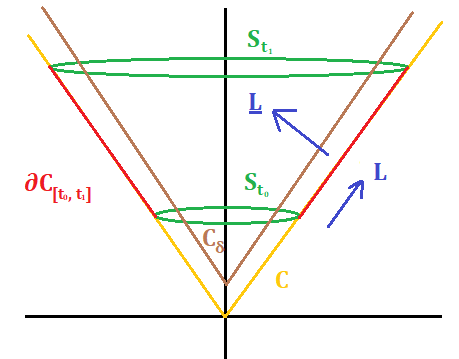
\includegraphics{graphics/cone}
			\caption{The geometry of the light cone. As a wise man once said, a picture is worth $\tfrac1\epsilon$-words for $\epsilon \ll 1$. }
		\end{center}	
	\end{figure}		

\subsubsection*{Subsets of $\R^d$ and $\R^{1 + d}$}
Define the restriction of the light cone to a time interval $I \subseteq [0, \infty)$ and a time slice $t \in [0, \infty)$ respectively by
	\begin{align*}
		C_I 
			&:= C \cap (I \times \R^d), \\
		S_{t}
			&:= C \cap (\{t\} \times \R^d).
	\end{align*}
The \emph{null boundary} $\partial C_I$ denotes the boundary of the time-slab $C_I$ modulo the top and bottom time-slices. Due to singularities on the null boundary, we will also consider the shifted light cone 
	\[ C^\delta := (\delta, 0) + C. \]
Accordingly, we have 
	\begin{align*}
		C^\delta_I
			&:= C_I \cap C^\delta, \\
		S^\delta_t
			&:= S_t \cap C^\delta.		
	\end{align*}	
We also define $B_r (x) \subseteq \R^d$ to be the ball of radius $r$ centered at $x$. 



\section{Conservation laws}

The non-linear wave equation \eqref{NLW} is the Euler-Lagrange equation arising when one formally considers solutions as critical points of the Lagrangian
	\[
		\cS[\phi] 
			:= \int_{\R^{1 + d}} \frac12 \partial_\alpha \phi \partial^\alpha \phi + \frac{d - 2}{2d} |\phi|^{\frac{2d}{d - 2}} \, dt dx.
	\]
By Noether's principle, the continuous symmetries of the equation lead to conserved quantities. We present the energy-momentum tensor formalism, which is derived from the diffeomorphism-invariance of the Lagrangian. Define the \emph{energy-momentum tensor} by
	\[
		T_{\mu \nu} 
			= \partial_\mu \phi \partial_\nu \phi - m_{\mu \nu} \left( \frac12 \partial_\alpha \phi \partial^\alpha \phi + \frac{d - 2}{2d} |\phi|^{\frac{2d}{d - 2}}  \right).
	\]	
Observe that $T_{\mu \nu}$ is a symmetric $2$-tensor. Furthermore, if $\phi$ is a classical solution to \eqref{NLW}, the energy-momentum tensor is also divergence-free, 
	\[
		\nabla^\mu T_{\mu \nu} = 0.
	\]
We obtain energy identities for the non-linear wave equation by contracting the energy-momentum tensor with well-chosen vector fields, and then integrate over suitable space-time domains. Given a vector field $X$, we define its deformation tensor to be the Lie derivative of the metric with respect to $X$, i.e. $^{(X)} \pi = \cL_X \bfm$. In coordinates, 
	\[
		^{(X)} \pi_{\mu \nu} = \partial_\mu X_\nu + \partial_\nu X_\mu. 
	\]
Define the $1$- and $0$-currents
	\begin{align*}
		^{(X)} J_\mu [\phi]
			&:= T_{\mu \nu} [\phi] X^\nu, \\
		^{(X)} K[\phi]
			&:= T_{\mu \nu} [\phi] \left(\frac12 {^{(X)}} \pi^\# \right)^{\mu \nu}.
	\end{align*}	
Then, since $T$ is divergence-free,
	\begin{equation}\tag{$\nabla$}\label{eq:current}
		\partial^\mu \left({^{(X)}} J_\mu [\phi] \right) = {^{(X)}} K[\phi].
	\end{equation}	
Another way of deriving the divergence identity above would be to multiply the equation \eqref{NLW} by $X\phi$ and then integrating-by-parts.\footnote{Well, technically, ``differentiating-by-parts''} More generally, we can apply the same procedure after multiplying the equation by $w\phi$ for a scalar weight $w$. It follows that the \emph{generalised $0$- and $1$-currents}
	\begin{align*}
		^{(X)} J_\mu [\phi]
			&:=w \phi \partial_\mu \phi - \frac12 \partial_\mu w |\phi|^2, \\
		^{(X)} K[\phi]
			&:= w \partial_\mu \phi \partial^\mu \phi - \frac12 \Box w |\phi|^2 + \kappa |\phi|^{p + 1} w,
	\end{align*}	
satisfy the divergence identity
	\begin{equation}\tag{$\nabla'$}\label{eq:gcurrent}
		\partial^\mu \left({^{(w)}} J_\mu [\phi] \right) = {^{(w)}} K[\phi].
	\end{equation}	
	
	
\subsection{Energy conservation identities}
	
The simplest conservation law arises from the stationarity of the Minkowski metric, that is, the time-like vector field $T = \partial_t$ is a Killing vector field, $^{(T)} \pi = 0$. Contracting the energy-momentum tensor with $T$, the resulting $1$-current is precisely the energy density
	\[
		^{(T)} J_\mu [\phi]
			= \frac12 |\partial_t \phi|^2 + \frac12 |\nabla \phi|^2 + \frac{d - 2}{2d} |\phi|^{\frac{2d}{d - 2}} .
	\]
Integrating the divergence identity \eqref{current} with $X = T$ over the space-time slab $(t_0, t_1) \times \R^d$ and applying the divergence theorem yields the conservation of energy,	

\begin{proposition}[Conservation of energy]
	Let $\phi \in C^0_{t, \loc} \dot H^1_x \cap \dot C^1_{t, \loc} L^2_x (I \times \R^d)$ be a strong solution to \eqref{NLW}, then the energy is conserved, i.e. $\cE[\phi[t]] \equiv \cE$ for all $t \in I$. 
\end{proposition}
	
To make full use of the finite speed of propagation and small data theory, as we will soon see in Section \ref{sec:local}, we need to derive an energy conservation law which is local in space. Given an open subset $\Omega \subseteq \R^d$, define the local energy on $\Omega$ at time $t$ by
	\[
		\cE_\Omega [\phi[t]] 
			:= \int_\Omega \frac12 |\partial_t \phi|^2 + \frac12 |\nabla \phi|^2 +  \frac{d - 2}{2d} |\phi|^{\frac{2d}{d - 2}} \, dx.
	\]	
We also write $\cE_{S_t} [\phi] := \cE_{B_t} [\phi[t]]$. Then, integrating \eqref{current} over the slab of the light-cone $C_{[t_0, t_1]}$ and applying the divergence theorem, we relate the local energy on the time-slices of the light cone $S_{t_0}$ and $S_{t_1}$ modulo a flux through the null boundary $\partial C_{[t_0, t_1]}$. To compute this flux, we write the $1$-current in null coordinates, remarking that $T = \tfrac12 (L + \underline L)$, 
	\begin{align*}
		{^{(T)}} J_L [\phi]
			&= \frac12 |L\phi|^2 + \frac12 |\slashed \nabla \phi|^2 +\frac{d - 2}{2d} |\phi|^{\frac{2d}{d - 2}} ,\\
		{^{(T)}} J_{\underline L} [\phi]
			&= \frac12 |\underline L\phi|^2 + \frac12 |\slashed \nabla \phi|^2 +\frac{d - 2}{2d} |\phi|^{\frac{2d}{d - 2}} .	
	\end{align*}
Thus, the flux through the null boundary takes the form 
	\[
		\cF_{\partial C_{[t_0, t_1]}} [\phi]
			:= \int_{\partial C_{[t_0, t_1]}} \left( \frac12 |L \phi|^2 + \frac12 |\slashed \nabla \phi|^2 + \frac{d - 2}{2d} |\phi|^{\frac{2d}{d - 2}}  \right) dS.
	\]
In summary, we obtain the following local energy conservation law, 




\begin{proposition}[Energy-flux identity]\label{prop:energyflux}
	Let $\phi \in C^0_{t, \loc} \dot H^1_x \cap \dot C^1_{t, \loc} L^2_x (I \times \R^d)$ be a strong solution to \eqref{NLW}, then the local energy and flux obey the identity
		\[
			\cF_{\partial C_{[t_0, t_1]}} [\phi] := \cE_{S_{t_1}} [\phi] - \cE_{S_{t_0}} [\phi].
		\]
\end{proposition}

Observe that the flux through the null boundary is non-negative. This implies that the local energy $\cE_{S_t} [\phi]$ in the light cone is non-decreasing as $t \uparrow \infty$ and non-increasing as $t \downarrow 0$. Since we are working with finite energy solutions, it follows from monotone convergence that the limits
	\begin{align*}
		\cE_0
			&:=\lim_{t \downarrow 0} \cE_{S_t} [\phi],\\
		\cE_\infty
			&:= \lim_{t \uparrow \infty} \cE_{S_t} [\phi],
	\end{align*}
exist. The former will be relevant for our discussion of the blow-up scenario; we defer the discussion to Section \ref{sec:local}. For now, we observe that the existence of the limits implies that

\begin{corollary}[Flux decay property]\label{cor:fluxdecay}
	Let $\phi \in C^0_{t, \loc} \dot H^1_x \cap \dot C^1_{t, \loc} L^2_x (I \times \R^d)$ be a strong solution to \eqref{NLW}, then the flux through the light cone vanishes at the tip and at infinity, 
		\begin{align*}
			\lim_{t_0, t_1 \downarrow 0} \cF_{\partial C_{[t_0, t_1]}} [\phi]
				&= 0, \\
			\lim_{t_0, t_1 \uparrow \infty} \cF_{\partial C_{[t_0, t_1]}} [\phi] 
				&= 0.	
		\end{align*}
\end{corollary}

As a corollary, we can show that the local energy on the exterior annuli $B_{B_{3t} \setminus B_t}[\phi[t]]$ decays as $t\downarrow 0$, 

\begin{figure}[h]
	\begin{center}
		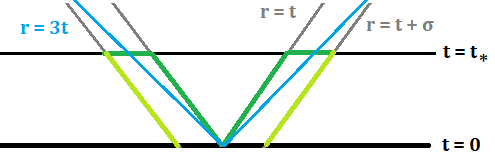
\includegraphics{graphics/exterior}
		\caption{We first choose, via flux decay, a time $t = t_*$ below which the flux is small, and then, via monotone convergence, $\sigma \ll 1$ such that the local energy in the annulus $B_{t_* + \sigma} \setminus B_{t_*}$ at time $t = t_*$ is small. The flux on the exterior cone has the correct sign, so we conclude from the energy-flux identity that the local energy in the annulus is small as $t \downarrow 0$. }
	\end{center}
\end{figure}

\begin{corollary}[Exterior energy decay]\label{cor:exterior}
	Let $\phi \in C^0_{t} \dot H^1_x \cap \dot C^1_{t} L^2_x ((0, 1] \times \R^d)$ be a finite energy local solution to \eqref{NLW}, then
		\[
			\lim_{\sigma \to 0} \limsup_{t \downarrow 0} \cE_{B_{t + \sigma} \setminus B_{t}} [\phi[t]] = 0.
		\]
	In particular, 
		\[
			\limsup_{t \downarrow 0} \cE_{B_{3t} \setminus B_{t}} [\phi[t]] = 0.
		\]	
\end{corollary}

\begin{proof}
	It is clear that for each $\sigma > 0$, we have $B_{3t} \setminus B_t \subseteq B_{t + \sigma} \setminus B_t$ for $t \ll \sigma$, which shows the latter decay statement is implied by the former. To prove the former, let $\epsilon > 0$, we choose from flux decay a time $t_* \ll 1$ such that
		\[
			\cF_{\partial C_{(0, t_*]}} [\phi] \ll \epsilon. 
		\]
	Then, considering the solution on the time slice $t = t_*$, it follows from monotone convergence that there exists $\sigma \ll 1$ such that 
		\[
			\cE_{B_{t_* + \sigma} \setminus B_{t_*}} [\phi[t_*]] \ll \epsilon.
		\]	
	It follows then from the energy-flux identity that, for $t \ll t_*$, 
		\begin{align*}
			 \cE_{B_{t + \sigma} \setminus B_{t}} [\phi[t]] 
			 	&= \cE_{B_{t + \sigma}} [\phi[t]] - \cE_{B_{t}} [\phi[t]] \\
			 	&= \left(\cE_{B_{t_* + \sigma}} [\phi[t_*]] - \cF_{- \sigma + \partial C_{[t, t_*]}} [\phi] \right) - \left( \cE_{B_{t_*}} [\phi[t_*]] - \cF_{\partial C_{[t, t_*]}} [\phi] \right).
		\end{align*}
	Since the flux is non-negative, we can throw away the first flux term, while by our choice of $t_* \ll 1$ and $\sigma \ll 1$ the exterior energy and flux at time $t = t_*$ is small,
		\[
			 \cE_{B_{t + \sigma} \setminus B_{t}} [\phi[t]] \leq  \cE_{B_{t_* + \sigma} \setminus B_{t_*}} [\phi[t_*]] + \cF_{\partial C_{(0, t_*]}} [\phi] \ll \epsilon.  
		\]
	This proves the result.
\end{proof}



\subsection{Monotonicity formula}

We derive a monotonicity formula for the non-linear wave equation arising from the scaling symmetry. The infinitesimal generator of this symmetry is given by $\Lambda = \partial_\rho + \tfrac1\rho$, so, after translating in time $t \mapsto t + \epsilon$ to handle the degeneracy at the light cone, we define 
	\begin{align*}
		X_\epsilon
			&= \frac{1}{\rho_\epsilon} ((t + \epsilon) \partial_t + r \partial_r), \\
		w_\epsilon
			&= \frac{d - 2}{2 \rho_\epsilon},	
	\end{align*}
where $\rho_\epsilon := \sqrt{(t + \epsilon)^2 - r^2}$. Observe that $X_0 = \tfrac1\rho S = \partial_\rho$, where $S$ is the scaling vector field. 
\begin{lemma}[Local monotonicity formula]
	Let $\phi$ be a smooth solution to \eqref{NLW} on an open subset $\cO \subseteq C_{(0, \infty)}$ of the forward light cone. Then the $1$-current defined in null coordinates by 
		\begin{align*}
			{^{(X_\epsilon)}} P_L [\phi]
				&= \frac12 \left( \frac{v_\epsilon}{u_\epsilon} \right)^{1/2} \left| r^{-\frac{d - 2}{2}} L \left( r^{\frac{d - 2}{2}} \phi \right)\right|^2 + \frac12 \left( \frac{u_\epsilon}{v_\epsilon} \right)^\frac12 \left( |\slashed \nabla \phi|^2 + \frac{(d - 2)^2}{4} \frac1{r^2} |\phi|^2 + \frac{d - 2}{d} |\phi|^{\frac{2d}{d - 2}} \right),\\
			{^{(X_\epsilon)}} P_{\underline L} [\phi]
				&= \frac12 \left( \frac{u_\epsilon}{v_\epsilon} \right)^{1/2} \left| r^{-\frac{d - 2}{2}} \underline L \left( r^{\frac{d - 2}{2}} \phi \right)\right|^2 + \frac12 \left( \frac{v_\epsilon}{u_\epsilon} \right)^\frac12 \left(  |\slashed \nabla \phi|^2 + \frac{(d - 2)^2}{4} \frac1{r^2} |\phi|^2 + \frac{d - 2}{d} |\phi|^{\frac{2d}{d - 2}}  \right),
		\end{align*}	
	setting the other components to zero, obeys the divergence identity
		\[
			\partial^\mu \left( {^{(X_\epsilon)}} P_\mu [\phi] \right) = \frac{1}{\rho_\epsilon} \left| \left( \partial_{\rho_\epsilon} + \frac1{\rho_\epsilon} \right)\phi \right|^2.
		\]	
\end{lemma}

\begin{proof}
	See Appendix \ref{app:A}
\end{proof}

Suppose the flux $\cF_{\partial C_{[t_0, t_1]}}[\phi]$ through the null boundary vanishes, then it follows that $\phi$ must also vanish along the null boundary. This kills the null boundary terms when we integrate the local monotonicity formula over the cone $C_{[t_0, t_1]}$ and apply the divergence theorem, thereby furnishing the identity
	\[
			\cM_{S_{t_1}} [\phi] + \iint_{C_{[t_0, t_1]}} \frac1\rho \left| \left( \partial_\rho + \frac1\rho \right) \phi\right|^2 \, dt dx = \cM_{S_{t_0}} [\phi],
	\]
for the weighted energy
	\begin{align*}
		\cM^\epsilon_{S_t} [\phi] 
			&:= \int_{S_t} {^{(X_\epsilon)}}P_T [\phi] \, dx \\
			&= \frac12 \int_{S_t} \left( \frac{v_\epsilon}{u_\epsilon} \right)^{1/2} \left| r^{-\frac{d - 2}{2}} \underline L \left( r^{\frac{d - 2}{2}} \phi \right)\right|^2 + \left( \frac{u_\epsilon}{v_\epsilon} \right)^{1/2} \left| r^{-\frac{d - 2}{2}} L \left( r^{\frac{d - 2}{2}} \phi \right)\right|^2 \\
			&\qquad + \left( \left( \frac{v_\epsilon}{u_\epsilon}\right)^\frac12  + \left( \frac{u_\epsilon}{v_\epsilon} \right)^\frac12 \right) \left(  |\slashed \nabla \phi|^2 + \frac{(d - 2)^2}{4} \frac1{r^2} |\phi|^2 + \frac{d - 2}{d} |\phi|^{\frac{2d}{d - 2}}  \right)	dx.
	\end{align*}
Since the second term is non-negative, this implies monotonocity of $\cM_{S_{t}}[\phi]$. In particular, the second term vanishes as $t_0, t_1 \to 0$, implying that rescalings of $\phi$ are asymptotically self-similar. On the other hand, the weights $(\tfrac{v}{u})^{1/2}$ blow-up at the null boundary, so there cannot be null concentration of energy. In the case where the flux does not vanish, we can still prove an "almost" monotonicity formula, leveraging the flux decay and a local Hardy's inequality to control the $\tfrac{|\phi|^2}{r^2}$ terms in the weighted energy. Before stating the almost monotonicity formula, we state and prove this Hardy decay. Define 
	\[
		\cG_{\partial S_t} [\phi]
			:= \frac1t \int_{\partial S_t} |\phi|^2.
	\]
This is well-defined for finite-energy solutions by the Sobolev trace theorem; in fact, $\phi \in H^{1/2}(\partial S_t)$.  

\begin{proposition}[Local Hardy's inequality]
	Let $\phi \in C^0_{t, \loc} \dot H^1_x \cap \dot C^1_{t, \loc} L^2_x (I \times \R^d)$, then
		\[
			\cG_{\partial S_{t_0}} [\phi] + \int_{t_0}^{t_1} \cG_{\partial S_t} [\phi] \frac{dt}{t} \leq \cG_{\partial S_{t_1}} [\phi] + \cF_{\partial C_{[t_0, t_1]}} [\phi].
		\]
	and 
		\[
			\cG_{\partial S_t} [\phi] \leq \cE_{\{t\} \times \R^d \setminus S_t} [\phi].
		\]		
\end{proposition}

\begin{proof}
	Standard proof of Hardy's inequality adapted to the null cone. 
\end{proof}

\begin{corollary}[Decay of Hardy term]
	Let $\phi \in C^0_{t, \loc} \dot H^1_x \cap \dot C^1_{t, \loc} L^2_x (I \times \R^d)$ be a strong solution to \eqref{NLW}, then $\cG_{\partial S_t} [\phi]$ vanishes as $t \to 0$ and $t \to \infty$,
		\begin{align*}
			\lim_{t \downarrow 0}\cG_{\partial S_t} [\phi]
				&= 0, \\
			\lim_{t \uparrow \infty}\cG_{\partial S_t} [\phi]
				&= 0.	
		\end{align*}	
\end{corollary}

\begin{proof}
	The local Hardy's inequality and finite energy implies that $\int \tfrac1t \cG_{\partial S_t} [\phi] < \infty$. We claim that if $\cG_{\partial S_t} [\phi]$ does not decay as $t\downarrow 0$ or $t\uparrow \infty$, then we can extract a uniform lower bound for either $t \ll 1$ or $t \gg 1$ respectively, a contradiction since $\int \tfrac1t$ diverges logarithmically. Suppose the $t \downarrow 0$ case fails; the case $t \uparrow \infty$ is similar, then local Hardy implies
		\[
			0 < \limsup_{t \downarrow 0} \cG_{\partial S_t} [\phi] \leq \cG_{S_t} [\phi] + \cF_{\partial C_{[0, t]}}.
		\]
	By flux decay, the flux term can be absorbed into the left-hand side for $t \ll 1$, proving the claim. 
\end{proof}

\begin{theorem}[Almost monotonicity formula I]\label{thm:monotone1}
	Let $\phi$ be a strong solution to \eqref{NLW} on $[\epsilon, 1] \times \R^d$ with negligible flux through the null boundary, finite energy and negligible Hardy term at $t = 1$, 
	\begin{align*}
		\cE_{S_1} [\phi]
			&\leq \cE, \\
		\cF_{\partial C_{[\epsilon, 1]}} [\phi]
			&\leq \epsilon^{1/2} \cE, \\
		\cG_{\partial S_1}[\phi]
			&\leq \epsilon^{1/2}\cE.
	\end{align*} 
	Then
		\[
			\cM_{S_{1}}^\epsilon [\phi] + \iint_{C_{[\epsilon, 1]}} \frac1{\rho_\epsilon} \left| \left( \partial_{\rho_\epsilon} + \frac1{\rho_\epsilon} \right) \phi\right|^2 \, dt dx \lesssim \cE.
		\]	
\end{theorem}

\begin{proof}
	Approximating a strong solution in the energy topology, it suffices to consider smooth solutions. We integrate the local monotonicity formula over the cone $C_{[\epsilon, 1]}$ and apply the divergence theorem, 
		\begin{align*}
			\cM_{S_{1}}^\epsilon [\phi] + \iint_{C_{[\epsilon, 1]}} \frac1{\rho_\epsilon} \left| \left( \partial_{\rho_\epsilon} + \frac1{\rho_\epsilon} \right) \phi\right|^2 \, dt dx 
				&=\cM_{S_{\epsilon}}^\epsilon [\phi] + \frac12 \int_{\partial C_{[\epsilon, 1]}} {^{(X_\epsilon)}}P_L [\phi] \, dS.
		\end{align*}
	We claim that the right-hand side is controlled by $\cE$.
	
	To control the weighted energy $\cM^\epsilon_{S_\epsilon} [\phi]$ on the time slice $S_\epsilon$, we first note that the weights can be treated as constants $|\tfrac{v_\epsilon}{u_\epsilon}| \sim |\tfrac{u_\epsilon}{v_\epsilon}| \sim 1$. It follows that we can estimate the integrand of the weighted energy $\cM^\epsilon_{S_\epsilon} [\phi]$ by the integrand of the local energy $\cE_{S_\epsilon} [\phi]$ and the Hardy term $\tfrac{|\phi|^2}{r^2}$, e.g.
		\begin{align*}
			\left(\frac{v_\epsilon}{u_\epsilon} \right)^{1/2} \left| r^{-\frac{d - 2}{2}} \underline L \left( r^{\frac{d - 2}{2}} \phi \right)\right|^2 + \left( \frac{u_\epsilon}{v_\epsilon} \right)^{1/2} \left| r^{-\frac{d - 2}{2}} L \left( r^{\frac{d - 2}{2}} \phi \right)\right|^2 
				&\lesssim  \left| r^{-\frac{d - 2}{2}} \underline L \left( r^{\frac{d - 2}{2}} \phi \right)\right|^2 + \left| r^{-\frac{d - 2}{2}} L \left( r^{\frac{d - 2}{2}} \phi \right)\right|^2 \\
				&\lesssim |\partial_t \phi|^2 + |\partial_r \phi|^2 + \frac{|\phi|^2}{r^2},
		\end{align*}
	and similarly for the other terms, so in total
		\[
			\cM^\epsilon_{S_\epsilon} [\phi] \lesssim \cE_{S_\epsilon} [\phi] + \int_{S_\epsilon} \frac{|\phi|^2}{r^2} \, dx \lesssim \cE
		\]	
	by finite energy, which controls $\cE_{S_\epsilon} [\phi]$, and negligible flux and Hardy term, which controls the right-hand side of the local Hardy's inequality. 

	To control the weighted flux term on the null boundary $\partial C_{[\epsilon, 1]}$, we observe that the weights are bounded above $|\tfrac{u_\epsilon}{v_\epsilon}| \leq 1$ and $|\tfrac{v_\epsilon}{u_\epsilon}| \lesssim \tfrac1\epsilon$ in this region. It follows that we can estimate the integrand of the weighted flux by the integrand of the usual flux $\cF_{[\epsilon, 1]}[\phi]$ and the Hardy term $\tfrac{|\phi|^2}{r^2}$, e.g.
		\begin{align*}
			^{(X_\epsilon)} P_L [\phi] \lesssim \epsilon^{-1/2} \left( |L\phi|^2 + \frac{|\phi|^2}{r^2} \right) + {^{(T)}} J_L [\phi],
		\end{align*}
	on the null boundary $\partial C_{[\epsilon, 1]}$, so integrating and applying the negligible flux and Hardy assumptions, 
		\[
			\int_{\partial C_{[\epsilon, 1]}} {^{(X_\epsilon)}} P_L [\phi] \, dS \lesssim \cE.
		\]	
	This completes the proof. 	
\end{proof}


\begin{corollary}[Almost monotonicity formula II]\label{thm:monotone2}
	Let $\phi$ be a strong solution to \eqref{NLW} on $[\epsilon, 1] \times \R^d$ satisfying the hypotheses of Theorem \ref{thm:monotone1}. Then
		\[
			\cM_{S^{\delta_1}_1} [\phi] \lesssim \cM_{S^{\delta_0}_{t_0}} [\phi] + \left( \left( \frac{\delta_1}{t_0}\right)^{1/2} + \frac{1}{|\log (\delta_1/\delta_0)|} \right) \cE
		\]	
	whenever $2\epsilon \leq \delta_0 \leq \delta_1 \leq t_0$. 	
\end{corollary}

\begin{proof}
	For any $\delta \in [\delta_0, \delta_1]$, we have that $S^{\delta_1}_1 \subseteq S^\delta_1$ and $S^{\delta_0}_{t_0} \subseteq S^{\delta}_{t_0}$. Thus, integrating the local monotonicity formula over the translated cone $C^\delta_{[t_0, 1]}$ and applying the divergence theorem, we see that it suffices to control the flux term 
		\[
			\int_{\partial C^\delta_{[t_0, 1]}} {^{(X)}} P_L [\phi] \, dS \lesssim  \left( \left( \frac{\delta_1}{t_0}\right)^{1/2} + \frac{1}{|\log (\delta_1/\delta_0)|} \right) \cE
		\]
	for appropriately chosen $\delta$. We control the term with $\tfrac{u}{v}$ weight by localised Hardy and local conservation of energy, 
		\begin{align*}
			\int_{\partial C^\delta_{[t_0, 1]}} &\left( \frac{u}{v} \right)^\frac12 \left( |\slashed \nabla \phi|^2 + \frac{(d - 2)^2}{4} \frac1{r^2} |\phi|^2 + \frac{d - 2}{d} |\phi|^{\frac{2d}{d - 2}} \right) dS\\
				 &\lesssim \left( \frac{\delta_1}{t_0} \right)^{1/2} \left( \cF_{\partial C^\delta_{[t_0, 1]}} [\phi] + \cE_{S_1 \setminus S_1^\delta} [\phi] + \cG_{S_1} [\phi]  \right) \lesssim  \left( \frac{\delta_1}{t_0} \right)^{1/2} \cE. 
		\end{align*}
	To treat the term with $\tfrac{v}{u}$ weight, we compute
		\[
			r^{-\frac{d - 2}{2}} L\left( r^{\frac{d- 2}{2}} \phi \right) = \left( L + \frac{d - 2}{2}\frac1r \right) \phi.
		\]	
	Finite energy plus pigeonhole principle. 	
\end{proof}

\section{Localising to the light cone}\label{sec:local}
Since the wave equation is time reversible, it suffices to consider the problem in one direction of time. To unify the notation, we consider the global well-posedness problem starting at time $t = 1$ backwards-in-time and the scattering problem starting at time $t = 0$ forwards-in-time. Assume towards a contradiction that the theorem fails, e.g. $\phi$ is a solution on $t \in (0, 1]$ blowing up as $t \downarrow 0$ or a global solution on $t \in[0, \infty)$ which fails to scatter $||\phi||_{\sfS[0, \infty)} = +\infty$. We claim that, after translating and rescaling, it suffices to consider solution which are regular outside of the forward light cone $C$, e.g.
	\begin{equation}\tag{$\epsilon_*$}\label{eq:exterior}
		\cE_{(\{t\} \times \R^3) \setminus S_t} [\phi[t]] \leq \epsilon_*.
	\end{equation}
This follows from the small data theory, smooth localisation of the energy, finite speed of propagation, and energy-flux decay. 

\subsection{Non-scattering scenario}

Suppose towards a contradiction that given finite energy data at time $t = 0$ the solution is global yet fails to scatter as $t \to \infty$. We localise by remarking that the energy-flux identity implies the energy exterior to a large light cone remains small for all time, and so the solution can be regarded as regular in view of small data theory. Indeed, by monotone convergence we can find a large ball $B_{R_*} \subseteq \R^d$ outside of which the energy of the initial data is arbitrarily small, 
	\[
		\cE_{\R^d \setminus B_{R_*}}[\phi[0]] \ll \epsilon_*. 
	\]
Recall that the energy-flux identity implies that the local energy $\cE_{S_t} [\phi]$ is non-decreasing, or, equivalently, the exterior energy $\cE_{\R^d \setminus S_t} [\phi]$ is non-increasing, as $t \to \infty$. Translating in time so that our solution starts at time $t = R_*$, we may assume the solution obeys
	\[
		\cE_{(\{t\} \times \R^3) \setminus S_t} [\phi] \ll \epsilon_*,
	\]
for all $t \in [R_*, \infty)$. To localise the solution to this exterior region, we will need finite speed of propagation and the following smooth cut-off lemma, 

\begin{lemma}[Exterior energy localisation]\label{lem:ext}
	Fix a cut-off $\chi \in C^\infty_c (\R^d)$ supported on the unit ball $|x| \leq 2$ and such that $\chi \equiv 1$ on the ball $|x| \leq 1$. Denote the rescalings $\chi_\lambda (x) := \chi(x/\lambda)$, then 
		\[
			||\nabla ((1 - \chi_\lambda) \phi)||_{L^2 (\R^d)}
				\lesssim_{d, ||\chi||_{L^\infty}, ||\nabla \chi||_{L^\infty}} ||\phi||_{L^{\frac{2d}{d - 2}} (|x| \geq  \lambda)} + ||\nabla \phi||_{L^2 (|x| \geq  \lambda)}
		\]
	uniformly in $\lambda > 0$. 	
\end{lemma}

\begin{proof}
	Computing the gradient of $\nabla ((1-\chi_\lambda) \phi)$ using the product and chain rules, and then applying the triangle inequality to the $L^2$-norm gives 
		\begin{align*}
			||\nabla ((1- \chi_\lambda)) \phi) ||_{L^2 (\R^d)} 
				&\leq \lambda^{-1} ||\nabla \chi||_{L^\infty} || \phi||_{L^2 (\lambda \leq |x| \leq 2\lambda)} + ||\chi ||_{L^\infty} || \nabla \phi||_{L^2 (|x| \geq \lambda)} .
		\end{align*}
	Here we have observed that the gradient of $\chi$ is supported in the annulus $1 \leq |x| \leq 2$. To estimate the lower order term, we apply Holder's inequality,
		\begin{align*}
			 \lambda^{-1} || \phi||_{L^2 (\lambda \leq |x| \leq 2\lambda)}
			 	&\leq  |A|\,  ||\phi||_{L^{\frac{2d}{d - 2}} (\lambda \leq |x| \leq 2\lambda)},
		\end{align*}	
	where $|A|$ denotes the volume of the annulus $1 \leq |x| \leq 2$. This completes the proof. 
\end{proof}

Cutting off the data at time $t = R_*$ to this exterior region, we obtain a global small-energy solution $\phi^{\mathrm{reg}}$ to \eqref{NLW} which by finite speed of propagation agrees with $\phi$ in this exterior region. In particular, as will be relevant for our rescaling argument in Section \ref{sec:ED}, the energy dispersion norm must be large within the light cone. 


\subsection{Blow-up scenario}

Suppose towards a contradiction that given data at time $t = 1$ the solution blows-up backwards in time as one approaches $t \downarrow 0$. To localise this scenario, we show that blow-up occurs only if energy concentrates within a light cone, 


\begin{proposition}[Blow-up implies energy concentration]\label{prop:blowup}
	Suppose $\phi \in C^0_{t} \dot H^1_x \cap \dot C^1_{t} L^2_x ((0, 1] \times \R^d)$ is a solution to \eqref{NLW} which blows-up as $t\downarrow 0$. Then there exists $x_* \in \R^d$ such that 
		\[
			\limsup_{t \downarrow 0} \cE_{B_{t} (x_*)} [\phi[t]] \geq \epsilon_* 
		\]
	for some absolute constant $\epsilon_* > 0$. 	
\end{proposition}

Our strategy will be to show that if energy does not concentrate, then we can extend the solution uniformly backwards in time to $[-\delta, 1] \times \R^d$ by gluing together a finite number of regions where this can be done. We first start with an exterior region, choosing $R_* \gg 1$ such that 
	\[
		\cE_{\R^d \setminus B_{R_*}} [\phi[1]] \ll \epsilon_*.
	\]
Using the exterior energy localisation from Lemma \ref{lem:ext}, we obtain a global small-energy solution $\phi^{\mathrm{reg}}$ to \eqref{NLW} which by finite speed of propagation agrees with $\phi$ outside the ball $B_{R_* + 1}$ at time $t = 0$. In particular, $\phi$ can be extended backwards in the domain of dependence of the exterior region. If we can find an open cover of $B_{R_* + 2}$ at time $t = 0$ by regions where $\phi$ can be extended, then we can conclude the result by extracting a finite cover by compactness and finite speed of propagation. 

\begin{figure}[h]
	\begin{center}
		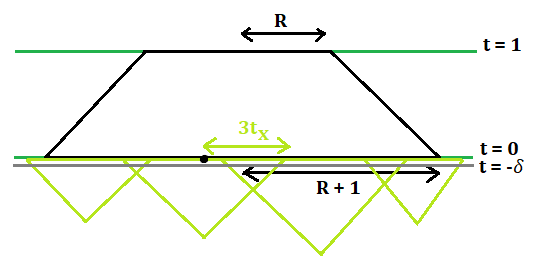
\includegraphics{graphics/blowup}
		\caption{The solution has small exterior energy and thus can be continued for some small time. If there is no energy concentration, we can cover the interior by a finite collection of light cones with small energy. Gluing together the local solutions, we can extend the whole solution uniformly in time. }
	\end{center}
\end{figure}	

By the exterior energy decay proved in Corollary \ref{cor:exterior}, it suffices to prove the result replacing the local energy in the light cone $\cE_{B_t (x_*)} [\phi[t]]$ with the energy in the larger cone $\cE_{B_{3t} (x_*)} [\phi[t]]$. Then, if energy does not concentrate, for each $x \in \R^d$ there exists $t_x \ll 1$ such that
	\[
		 \cE_{B_{3t_x} (x)} [\phi[t_x]] < \epsilon_*.
	\]	
To use the small data theory to rule out blow-up within the domain of dependence of, say, $B_{2t_x} (x)$ at time $t = t_x$, we need to localise in space, 

\begin{lemma}[Localisation of energy]\label{lem:local}
	Fix a cut-off $\chi \in C^\infty_c (\R^d)$ supported on the unit ball $|x| \leq 1$ and such that $\chi \equiv 1$ on the ball $|x| \leq \tfrac12$. Denote the rescalings $\chi_\lambda (x) := \chi(x/\lambda)$, then 
		\[
			||\nabla (\chi_\lambda \phi) ||_{L^2 (\R^d)} \lesssim_{d, ||\chi||_{L^\infty}, ||\nabla\chi||_{L^\infty}} ||\phi||_{L^{\frac{2d}{d - 2}} (|x|\leq \lambda)}  +  ||\nabla \phi||_{L^2 (|x| \leq \lambda)}.
		\]
\end{lemma}

\begin{proof}
	Computing the gradient of $\nabla (\chi_\lambda \phi)$ using the product and chain rules, and then applying the triangle inequality to the $L^2$-norm gives 
		\begin{align*}
			||\nabla (\chi_\lambda \phi) ||_{L^2 (\R^d)} 
				&\leq \lambda^{-1} ||\nabla \chi||_{L^\infty} || \phi||_{L^2 (|x| \leq \lambda)} + ||\chi ||_{L^\infty} || \nabla \phi||_{L^2 (|x| \leq \frac12 \lambda)} .
		\end{align*}
	To estimate the lower order term, we apply Holder's inequality,
		\begin{align*}
			 \lambda^{-1} || \phi||_{L^2 (|x| \leq \lambda)}
			 	&\leq  |B|\,  ||\phi||_{L^{\frac{2d}{d - 2}} (|x| \leq \lambda)},
		\end{align*}	
	where $|B|$ denotes the volume of the unit ball. This proves the result. 
\end{proof}

Applying the localisation lemma, we can apply a cut-off to obtain data $\phi^{\mathrm{reg}} [t_x]$ which has small energy and agrees with $\phi[t_x]$ on the ball $B_{2t_x} (x)$. By the small-data theory, the localised data admits a global solution $\phi^{\mathrm{reg}}$, while finite speed of propagation tells us that this solution agrees with $\phi$ in the domain of dependence of $B_{2t_x} (x)$ at time $t = t_x$. In particular, $\phi$ is regular in the ball $B_{t_x} (x)$ at time $t = 0$ and can be continued past this time. This completes the proof of Proposition \ref{prop:blowup}. That is, after translating in space, the solution blows up by concentrating energy inside a light cone towards the origin, 
	\[
		\limsup_{t \downarrow 0}\cE_{S_t} [\phi] \geq \epsilon_*. 
	\]
Following the proof of exterior energy decay, Corollary \ref{cor:exterior}, we can truncate the data at time $t_0 \ll 1$ so that the solution remains unchanged in the interior of the light cone $C_{[0, t_0]}$ and has small energy exterior to the light cone. We leave this as an exercise. 











\section{Concentration of energy}\label{sec:ED}
We now turn to the proof of quantitative regularity, Theorem \ref{thm:tao1}, in the critical space $L^\infty_t L^3_x ([0, T] \times \R^3)$. Throughout we will assume the solution satisfies the \emph{a priori} $L^\infty_t L^3_x$-bound 
	\begin{equation}
		||u||_{L^\infty_t L^3_x} 
			\leq A, \label{eq:apriori}
	\end{equation}
for some $A \geq C_0 \gg 1$. To give some motivation for the main stacking argument in Section \ref{sec:stack}, we first prove an ``energy-dispersion implies regularity''-type theorem. More precisely, we claim that if the solution does not concentrate in amplitude at small scales, then the solution must be regular. Before stating the theorem, we record a standard regularity lemma which will be useful throughout: 

\begin{lemma}\label{lem:prelim}
	Let $u: I \times \R^3 \to \R^3$ be a strong solution to \eqref{NS} which obeys an $L^\infty_t L^3_x$-bound \eqref{apriori}. Then 
		\begin{enumerate}
			\item if we had control over the subcritical quantities
			 \begin{align*}
			||\nabla u^\nlin||_{L^\infty_t L^2_x} 
				&\leq M,\\
			||\nabla^2 u^\nlin||_{L^2_{t, x}}
				&\leq M,
		\end{align*}
	then we have regularity, 
		\[
			||\nabla^j_x u(t)||_{L^\infty_x} \lesssim_A M^{c} t^{-\frac{j + 1}{2}}.
		\]
			
			\item we can bound supercritical quantities in terms of $A$, e.g.
				\[
					||u^\nlin||_{L^\infty_t L^2_x} + ||\nabla u^\nlin||_{L^2_{t, x}} \lesssim A^2.
				\]
		\end{enumerate}
\end{lemma}

\begin{remark}
	The splitting into linear and non-linear components of the solution is convenient since it is difficult to control $u^\lin$ in $L^2_x (\R^3)$, since parabolic smoothing only allows us to control it in higher $L^p_x$-spaces. 
\end{remark}

\begin{theorem}[``Energy-dispersed'' regularity theorem]
	Let $u: [0, T] \times \R^3 \to \R^3$ be a classical solution to the Navier-Stokes equations \eqref{NS} which obeys the a priori $L^\infty_t L^3_x$-bound \eqref{apriori}. Then there exists $\epsilon \ll 1$ and $N_* \gg_A 1$ such that if
		\[
			N^{-1} ||P_N u||_{L^\infty_{t, x}} < \epsilon
		\]
	for all $N_0 \geq N_*$, then 
		\[
			||\nabla^j_x u(t)||_{L^\infty_x} \lesssim N_*^{O(1)} t^{-\frac{j + 1}{2}}.
		\]
\end{theorem}

\begin{proof}
	By scaling, it suffices to consider the case $t = 1$. We split the velocity and vorticity fields into the linear components, $u^\lin := e^{t \Delta} u_0$ and $\omega^\lin := e^{t \Delta} \omega_0$, and non-linear components, $u = u^\lin + u^\nlin$ and $\omega = \omega^\lin + \omega^\nlin$. We argue by the energy method, defining the non-linear enstrophy
		\[
			E(t) := \frac12 \int_{\R^3} |\omega^\nlin (t, x)|^2 \,dx .
		\]
	We compute
		\[
			\partial_t E(t)
				= - Y_1 (t) + Y_2 (t) + Y_3 (t) + Y_4(t) + Y_5 (t),
		\]	
	where
		\begin{align*}
			Y_1 (t)
				&= \int_{\R^3} |\nabla \omega^\nlin|^2 \, dx, \\
			Y_2 (t)
				&=- \int_{\R^3} \omega^\nlin \cdot (u \cdot \nabla) \omega^\lin \, dx ,\\
			Y_3 (t)
				&= \int_{\R^3}\omega^\nlin \cdot (\omega^\nlin \cdot \nabla) u^\nlin \, dx, \\
			Y_4 (t)
				&= \int_{\R^3} \omega^\nlin \cdot (\omega^\nlin \cdot \nabla) u^\lin \, dx, \\
			Y_5 (t)
				&= \int_{\R^3} \omega^\nlin \cdot (\omega^\lin \cdot \nabla) u^\nlin \, dx, \\
			Y_6 (t)
				&= \int_{\R^3}\omega^\nlin \cdot (\omega^\lin \cdot \nabla) u^\lin \, dx.		
		\end{align*}	
	To conclude, we aim for control over the sub-critical quantities $E(t)$ and $\int Y_1 \, dt$. Applying parabolic smoothing and the a priori estimate \eqref{apriori} for the linear contributions, Holder's inequality gives
		\begin{align*}
			Y_2 (t), Y_6 (t)
				&\lesssim A^2 E(t)^{1/2} \lesssim A^4 + E(t), \\
			Y_4 (t), Y_5(t)
				&\lesssim A E(t). 	
		\end{align*}
	We use the non-concentration at high frequencies to handle the purely non-linear term $Y_3 (t)$. Performing a Littlewood-Paley decomposition, placing low frequencies in $L^\infty_x$ and high frequencies in $L^2_x$, we write
		\begin{align*}
			Y_3 (t)
				&\leq \sum_{N_1, N_2, N_3} \int_{\R^3} |P_{N_1} \omega^\nlin \cdot (P_{N_2} \omega^\nlin \cdot \nabla) P_{N_3} u^\nlin| \, dx \\
				&\lesssim \sum_{\substack{N_1, N_2, N_3 \\ N_1 \sim N_2 \gtrsim N_3} } ||P_{N_1} \omega^\nlin ||_{L^2_x}^2 ||P_{N_3} \omega^\nlin||_{L^\infty_x}.
		\end{align*}	
	We control the $L^\infty$-norm for frequencies $N_3 \leq N_*$ using the trivial bound coming from the a priori estimate \eqref{apriori} and Sobolev-Bernstein, while the non-concentration kicks in at frequencies $N_* \leq N_3 \lesssim N_2$. Thus, we can control the sum in $N_3$ by 
		\[
			\sum_{\substack{N_3 : N_3 \lesssim N_2}} ||P_{N_3} \omega^\nlin||_{L^\infty_x} \lesssim \epsilon N_2^2 + AN_*^2. 
		\]	
	Inserting this back into the estimate for $Y_3(t)$, using Cauchy Schwartz and Plancharel gives
		\[
			Y_3 (t) \lesssim \epsilon Y_1 (t) + AN_*^2 E(t).
		\]	
	Collecting our results and choosing $\epsilon \ll 1$ such that $\epsilon Y_1 (t)$ can be absorbed into the left-hand side, we obtain
		\[
			\partial_t E(t) + Y_1 (t) \lesssim AN_*^2 E(t) + A^4. 
		\]	
	It remains to prove the desired estimate for $E(t)$ on, e.g. the interval $[3/4, 1]$, as inserting the bound into the above and integrating would give the desired control over $\int Y_1 \, dt$. Applying Gronwall, 
		\[
			E(t_2) \lesssim E(t_1) + A^4
		\]	
	for $|t_2 - t_1| \leq A^{-1} N_*^{-2}$. On the other hand, we can control the supercritical quantity 
		\[
			\int_{1/2}^1 E(t) \lesssim A^4,
		\]	
	see Lemma \ref{lem:prelim}. Pigeonholing, we can find $E(t) \lesssim A^5 N_*^2$ in an interval of length $A^{-1} N_*^{-2}$. This can be extended by our Gronwall argument to $t \in [3/4, 1]$. Going back into our energy estimates, this controls $\int Y_1 \, dt$ as well, so we have enough sub-critical control to conclude the proof. 
\end{proof}

\begin{remark}
	One should compare with the energy dispersion implies regularity results for dispersive equations, e.g. wave maps \cite{SterbenzTataru2010a}, or the non-linear wave equation. However, in this context, it seems one needs smallness for all frequency scales, not just large frequencies. Essentially the argument boils down to applying the refined Sobolev inequality to control the non-linearity, allowing us to close the regularity argument with Strichartz. 
\end{remark}




\section{Bubbling off a soliton}


\begin{proposition}
	There exists a constant $\epsilon_0 > 0$ such that for every sequence $\{\phi_n\}_n$ of solutions to the defocusing \eqref{NLW} on $(-2, 2) \times 4B$ with uniformly small energy
		\begin{align}
			\cE_{\{0\} \times 4B} [\phi_n] 
				&\ll \epsilon_0^2, 
		\end{align}
	and is asymptotically stationary, 
		\begin{align}
			\iint_{(-2, 2) \times 4B} |(Y + b) \phi_n|^2 \, dx \overset{n \to \infty}{\longrightarrow} 0,
		\end{align}
	for some uniformly time-like vector field $Y$ and a smooth function $b$, then, after passing to a subsequence, we can extract a solution $\Phi \in H^{3/2}_{t, x} ((-1, 1) \times B)$ to the defocusing \eqref{NLW} to which the sequence converges strongly in $H^1 ((-1, 1) \times B)$ and 
		\begin{equation}
			(Y + b) \Phi = 0. 
		\end{equation}
		
\end{proposition} 
	
\begin{proof}
	
\end{proof}	


\section{Rigidity}


In our blow-up analysis, we showed that there are only two possibilities for energy concentration: either time-like concentration or self-similar concentration. Using the compactness lemma, we can extract either a stationary solution or a self-similar solution. Both are impossible, leading to a contradiction. 
	
\begin{proposition}[No non-trivial finite-energy stationary solutions]
	Let $\phi$ be a finite-energy smooth solution to the defocusing \eqref{NLW} on $\R^{1 + d}$ which is stationary, i.e. there exists a unit constant time-like vector field $Y$ such that $Y\phi = 0$. Then $\phi \equiv 0$. 
\end{proposition}	

\begin{proof}
	Any unit constant time-like vector field can be Lorentz transformed into the vector field $T = \partial_t$, so in particular we can write $Y \phi = \partial_t L_v \phi$ for some Lorentz transformation $L_v$. As these transformations commute with the wave operator $\Box$, it follows from stationarity that the Lorentz transformed solution satisfies the elliptic equation
		\[
			\Delta L_v \phi = \Box L_v \phi = L_v \Box \phi = L_v \left( |\phi|^{p - 1} \phi\right) = |L_v \phi|^{p - 1} L_v \phi. 
		\]
	Writing $Q = L_v \phi$, multiply the equation by $Q$ and integrate to obtain 
		\[
			 \int_{\R^d} Q \Delta Q \, dx = \int_{\R^d} |Q|^{p + 1} \, dx.
		\]
	Integrating the left-hand side by parts, we see that it is non-positive, while the right-hand side is non-negative. We conclude $Q \equiv 0$.	
\end{proof}

\begin{proposition}[No non-trivial finite-energy self-similar solutions]
	Let $\phi$ be a finite-energy smooth solution to the defocusing \eqref{NLW} on the forward light cone $C_{(0, \infty)}$ which is self-similar, i.e. $(\partial_\rho + \tfrac1\rho) \phi = 0$. Then $\phi \equiv 0$. 
\end{proposition}

\begin{proof}
	Writing in hyperbolic coordinates $\Box = -\rho^{-d} \partial_\rho \rho^d \partial_\rho + \rho^{-2} \Delta_{\HH^d}$, we compute 
		\begin{align*}
			\Box \phi 
				&= - \rho^{-d} \partial_\rho \left( \rho^d \partial_\rho \phi \right) + \rho^{-2}\Delta_{\HH^d} \phi \\
				&=  \rho^{-d} \partial_\rho (\rho^{d - 1} \phi) +  \rho^{-2}\Delta_{\HH^d} \phi \\
				&= \left( (d - 1) \rho^{-2} \phi + \rho^{-1} \partial_\rho \phi \right) +  \rho^{-2}  \Delta_{\HH^d} \phi = \rho^{-2} \left( d - 2 +  \Delta_{\HH^d} \right) \phi. 
		\end{align*}
	Thus $\phi$ solves the elliptic equation 
		\[
			(d - 2 + \Delta_{\HH^d}) \phi = \rho^2 |\phi|^{p - 1} \phi. 
		\]	
	Since $\phi$ is finite-energy, we know that $\phi \in \dot H^1 (\HH^d_\rho)$ on each hyperboloid; we leave this as an exercise. As with the case of stationary solutions, multiplying the equation by $\phi$, integrating on $\HH^d$, and integrating-by-parts furnishes the result. 
\end{proof}

\begin{remark}
	Recall self-similar coordinates for the non-linear wave equation are given by 
		\[
			\rho = \sqrt{t^2 - r^2}, \qquad \xi = \frac{|x|}{|t|}.
		\]
	The Minkowski metric can be expressed in these coordinates as 
		\[
			\bfm = - d \rho^2 + \rho^2 \left( \frac{d \xi^2}{(1 - \xi^2)^2} + \frac{\xi^2}{1 - \xi^2} g_{\SS^{d - 1}}\right).
		\]	
	In particular $(\partial_\rho - \tfrac1\rho) \phi = 0$ implies that 
		\[
			\phi(t, x) = t^{-\frac{2}{p - 1}} W(x/t)
		\]
	for some self-similar profile $W$. In view of the scaling symmetries, this implies that the flux on any portion of the null boundary is the same. 		
\end{remark}

\appendix
\section{Derivation of monotonicity formula}\label{app:A}

We derive the key monotonicity formula associated to the scaling vector field. We follow a computation similar to that for Maxwell-Klein-Gordon \cite[Section 5]{OhTataru2016}. In view of the degeneracy of the light cone, we make a translation in time $t \mapsto t + \epsilon$, defining 
	\begin{align*}
		X_\epsilon
			&= \frac{1}{\rho_\epsilon^k} ((t + \epsilon) \partial_t + r \partial_r), \\
		w_\epsilon
			&= \frac{d - k - 1}{2 \rho^k_\epsilon},	
	\end{align*}
where $\rho_\epsilon := \sqrt{(t + \epsilon)^2 - r^2}$. In view of scaling, $k = d - 1 - \tfrac{4}{p - 1}$; we are interested in the NLW energy critical exponents, so $k = 1$. Observe that $X_0 = \tfrac1\rho S = \partial_\rho$, where $S$ is the scaling vector field. To simplify the discussion, we first restrict to the case $\epsilon = 0$. Translating in time, we will conclude


\begin{theorem}[Monotonicity formula]
	Let $\phi$ be a smooth solution to \eqref{NLW} on an open subset $\cO \subseteq C_{(0, \infty)}$ of the forward light cone. Then the $1$-current defined by 
		\begin{equation}
			^{(X_\epsilon)}P_\mu [\phi]
				= {^{(X_\epsilon)}} J_\mu [\phi] + {^{(w_\epsilon)}} J_\mu [\phi] + {^{(\cH_\epsilon)}} J_\mu [\phi] +  {^{(\cN_\epsilon)}} J_\mu [\phi]
		\end{equation}	
	satisfies the divergence identity
		\begin{equation}
			\partial^\mu \left( {^{(X_\epsilon)}} P_\mu [\phi] \right) = \frac{1}{\rho_\epsilon} \left| \left( \partial_{\rho_\epsilon} + \frac1{\rho_\epsilon} \right)\phi \right|^2.
		\end{equation}	
	In null coordinates,
		\begin{equation}
		\begin{split}
			{^{(X_\epsilon)}} P_L [\phi]
				&= \frac12 \left( \frac{v_\epsilon}{u_\epsilon} \right)^{1/2} \left| r^{-\frac{d - 2}{2}} L \left( r^{\frac{d - 2}{2}} \phi \right)\right|^2 + \frac12 \left( \frac{u_\epsilon}{v_\epsilon} \right)^\frac12 \left( |\slashed \nabla \phi|^2 + \frac{(d - 2)^2}{4} \frac1{r^2} |\phi|^2 + \frac{2\kappa}{p + 1} |\phi|^{p + 1} \right)\\
			{^{(X_\epsilon)}} P_{\underline L} [\phi]
				&= \frac12 \left( \frac{u_\epsilon}{v_\epsilon} \right)^{1/2} \left| r^{-\frac{d - 2}{2}} \underline L \left( r^{\frac{d - 2}{2}} \phi \right)\right|^2 + \frac12 \left( \frac{v_\epsilon}{u_\epsilon} \right)^\frac12 \left(  |\slashed \nabla \phi|^2 + \frac{(d - 2)^2}{4} \frac1{r^2} |\phi|^2 + \frac{2\kappa}{p + 1} |\phi|^{p + 1} \right)	.
		\end{split}	
		\end{equation}	
\end{theorem}

\subsubsection{$0$-current}

We first work in hyperbolic coordinates. Writing the metric in these coordinates, the Lie derivative of the metric along the coordinate vector field $\partial_\rho$ is given by $\cL_{\partial_\rho} \bfm = 2 \rho (\d y^2 + \sinh^2 (y) g_{\SS^{d - 1}})$. Thus, we can write the deformation tensor along $X_0$ as 
	\begin{align*}
		\frac12 {^{(X_0)}} \pi
			&= \rho (\d y^2 + \sinh^2 (y) g_{\SS^{d - 1}} \\
			&= \frac1\rho \d \rho^2 + \frac1\rho \bfm,	
	\end{align*}
with metric dual
	\begin{align*}
		\frac12 {^{(X_0)}} \pi^\# 
			&= \rho (\partial_y \odot \partial_y + \sinh^2 (y) g_{\SS^{d - 1}}^{-1} ) \\
			&= \frac1\rho \partial_\rho \odot \partial_\rho + \frac1\rho \bfm^{-1}. 	
	\end{align*}
The $0$-current is given by 
	\begin{align*}
		{^{(X_0)}} K[\phi]
			&= T[\phi] \left( \frac12 {^{(X_0)}} \pi^\#\right) \\
			&= \frac1\rho \left( T_{\rho \rho} + \operatorname{tr} T \right) \\
			&= \frac1\rho \left( |\partial_\rho \phi|^2 + \frac{2 - d}{2} |\nabla \phi|^2 - \kappa \frac{d - 2}{2} |\phi|^{\frac{2d}{d - 2}} \right).
	\end{align*}
For $d \geq 3$, the second term has bad sign. Furthermore, we want to rewrite the first term in terms of the infinitesimal generator of the scaling symmetry $\Lambda = \partial_\rho + \tfrac1\rho$. To remove the term with bad sign, we introduce the generalised current. The d'Alembertian of our weight is $-\tfrac12 \Box \tfrac1\rho = - \frac{d - 2}{2} \tfrac1{\rho^3}$, so the generalised $0$-current takes the form 
	\begin{align*}
		{^{(w_0)}} K[\phi]
			&= \frac{d - 2}{2\rho} |\nabla \phi|^2 - \frac{(d - 2)^2}{4} \frac{1}{\rho^3} |\phi|^2 + \kappa \frac{d - 2}{2 \rho} |\phi|^{\frac{2d}{d - 2}}\\
			&= \frac1\rho \left( \frac{d - 2}{2} |\nabla \phi|^2 - \frac{(d - 2)^2}{4} \left| \frac1\rho \phi\right|^2 + \kappa \frac{d - 2}{2} |\phi|^{\frac{2d}{d - 2}} \right).
	\end{align*}
It remains to handle the first term of $^{(X_0)} K[\phi]$ and the second term coming from $^{(w_0)} K[\phi]$. This will be done by Hardy's inequality, or, more descriptively, completing-the-square with integration-by-parts. Define the Hardy $0$- and $1$-currents 
	\begin{equation}
	\begin{split}
		{^{(\cH_0}} J_\rho [\phi]
			&:= - \frac{d - 2}{2\rho^2} |\phi|^2, \\
		{^{(\cH_0)}} K[\phi]
			&:= - \frac{(d - 2)^2}{2\rho^3} |\phi|^2 + \frac{d - 2}{2\rho^2} |\phi|^2\\
			&= \frac1\rho \left( \frac{(d -2)^2}{2} \left| \frac1\rho \phi \right|^2 + \frac{d - 2}{\rho^2} \phi \partial_\rho \phi \right)	.
	\end{split}		
	\end{equation}
We set the other components of $^{(\cH_0)} J[\phi$ to be zero. Then, using $\nabla^\mu ({^{(\cH_0)}} J_\mu  = - \rho^{-d} \partial_\rho (\rho^d ({^{(\cH_0)}} J_\rho  ))$, we obtain the divergence identity 
	\begin{equation}
		\nabla^\mu \left( {^{(\cH_0)}} J_\mu [\phi] \right) = {^{(\cH_0)}} K[\phi].
	\end{equation}
Collecting the $0$-curents, 
	\begin{align}
		{^{(X_0)}} K[\phi]
			&= \frac1\rho \left( |\partial_\rho \phi|^2 + \frac{2 - d}{2} |\nabla \phi|^2 - \kappa \frac{d - 2}{2} |\phi|^{\frac{2d}{d - 2}} \right),\\
		{^{(w_0)}} K[\phi]
			&= \frac1\rho \left( \frac{d - 2}{2} |\nabla \phi|^2 - \frac{(d - 2)^2}{4} \left| \frac1\rho \phi\right|^2 + \kappa \frac{d - 2}{2} |\phi|^{\frac{2d}{d - 2}} \right),\\
		{^{(\cH_0)}} K[\phi]
			&= \frac1\rho \left( \frac{(d - 2)^2}2 \left| \frac1\rho \phi\right|^2 + \frac{d - 2}{\rho^2} \phi \partial_\rho \phi \right),
	\end{align}
we write
	\begin{equation}
		 {^{(X_0)}} K[\phi] + {^{(w_0)}} K[\phi] + {^{(\cH_0)}} K[\phi] = \frac1\rho \left| \left( \partial_\rho + \frac{d - 2}{2 \rho} \right) \phi \right|^2.
	\end{equation}
\subsubsection{$1$-current}

Ideally we wold like for the flux term to have a sign. It is convenient here to work in null coordinates, so we perform a null decomposition. At each point $p = (t_0, x_0)$, consider an orthonormal frame $\{ e_\fra \}_{\fra = 1, \dots, d - 1}$ for the sphere $\{t_0\} \times \partial B_{\rho_0} (0)$. Then $\{L, \underline L, e_1, \dots, e_{d - 1}\}$ forms a null frame at $p$. We decompose $\nabla \phi$ with respect to the null frame into $L\phi$, $\underline L \phi$ and $\slashed \nabla_\fra \phi$,
	\begin{equation}
		\begin{split}
			T[\phi](L, \underline L)
				&= |L\phi|^2, \\
			T[\phi]	(\underline L, \underline L)
				&= |\underline L \phi|^2, \\
			T[\phi] (L, \underline L)
				&= |\slashed \nabla \phi|^2 + \kappa \frac{d - 2}{d} |\phi|^{\frac{2d}{d - 2}}.
		\end{split}
	\end{equation}
Furthermore, recall that 
	\[
		\rho^2 = uv, \qquad X_0 = \frac12 \left( \frac{v}{u} \right)^{1/2} L + \frac12 \left( \frac{u}{v} \right)^{1/2} \underline L. 
	\]
Then the $1$-currents in these coordinates take the form 
	\begin{equation}
	\begin{split}
		{^{(X_0)}} J_L [\phi]
			&= \frac12 \left( \frac{v}{u} \right)^{1/2}  |L \phi|^2 + \frac12 \left( \frac{u}{v}\right)^{1/2} \left( |\slashed \nabla \phi|^2 + \kappa \frac{d - 2}{d} |\phi|^{\frac{2d}{d - 2}}  \right),\\
		{^{(X_0)}} J_{\underline L} [\phi]
			&= \frac12 \left( \frac{u}{v} \right)^{1/2}  |\underline L \phi|^2 + \frac12 \left( \frac{v}{u}\right)^{1/2} \left( |\slashed \nabla \phi|^2 + \kappa \frac{d - 2}{d} |\phi|^{\frac{2d}{d - 2}}  \right)	
	\end{split}
	\end{equation}	
and
	\begin{equation}
	\begin{split}
		{^{(w_0)}} J_L [\phi]
			&= \frac{d - 2}{2\rho} \phi L\phi + \frac{d - 2}{4} \left( \frac{u}{v} \right)^{1/2} \frac1{\rho^2} |\phi|^2,\\ 
		{^{(w_0)}} J_{\underline L} [\phi]
			&= \frac{d - 2}{2\rho} \phi \underline L\phi + \frac{d - 2}{4} \left( \frac{v}{u} \right)^{1/2} \frac1{\rho^2} |\phi|^2	
	\end{split}
	\end{equation}		
and, writing $\d \rho = \tfrac12 \left(\tfrac{u}{v}\right)^{1/2} \d v + \tfrac12 \left( \tfrac{v}{u} \right)^{1/2} \d u$, 
	\begin{equation}
	\begin{split}
		{^{(\cH_0)}} J_L [\phi]
			&= - \frac{d -2}{2} \left( \frac{u}{v} \right)^{1/2} \frac1{\rho^2} |\phi|^2, \\
		{^{(\cH_0)}} J_L [\phi]
			&= - \frac{d -2}{2} \left( \frac{v}{u} \right)^{1/2} \frac1{\rho^2} |\phi|^2.	
	\end{split}
	\end{equation}
Evidently, adding these three expressions does not give a good sign. We complete the square again, computing 
	\begin{align*}
		\left| r^{- \frac{d - 2}{2}} L \left( r^{\frac{d - 2}{2}} \phi \right) \right|^2	
			&= |L\phi|^2 + \frac{d - 2}{r} \phi L \phi + \frac{(d - 2)^2}{4} \frac1{r^2} |\phi|^2, \\
		\left| r^{- \frac{d - 2}{2}}\underline L \left( r^{\frac{d - 2}{2}} \phi \right) \right|^2	
			&= |\underline L\phi|^2 - \frac{d - 2}{r} \phi L \phi + \frac{(d - 2)^2}{4} \frac1{r^2} |\phi|^2.
	\end{align*}	
The game then is to rewrite	
	\begin{align*}
		{\color{green} \frac{d - 2}{2\rho} \phi L \phi - \frac12 \left(\frac{v}{u} \right)^{1/2} \frac{d - 2}{r}  \phi L \phi}
			&= {\color{green} -\frac{d - 2}{2} \frac{t}{r \rho} \phi L \phi}, 
			\\
		{\color{green} \frac{d - 2}{2\rho}  \phi \underline L  \phi  + \frac12 \left(\frac{u}{v} \right)^{1/2} \frac{d - 2}{r}  \phi \underline L  \phi }
			&={\color{green} +\frac{d - 2}{2} \frac{t}{r \rho} \phi \underline L  \phi },
			\\
		{\color{red} -\frac{d - 2}{4} \left(  \frac{u}{v}\right)^{1/2} \frac{1}{\rho^2} |\phi|^2 - \frac12 \left(  \frac{v}{u}\right)^{1/2} \frac{(d - 2)^2}{4} \frac{1}{r^2} |\phi|^2 }	
			&= {\color{red} - \left(\frac{d - 2}{4}    \frac{1}{\rho v}  + \frac12  \frac{(d - 2)^2}{4} \frac{v}{r^2 \rho} \right) |\phi|^2},
			\\
		{\color{red} -\frac{d - 2}{4} \left(  \frac{v}{u}\right)^{1/2} \frac{1}{\rho^2} |\phi|^2 - \frac12 \left(  \frac{u}{v}\right)^{1/2} \frac{(d - 2)^2}{4} \frac{1}{r^2} |\phi|^2 }
			&= {\color{red}-\left( \frac{d - 2}{4}  \frac{1}{\rho u}  + \frac12 \frac{(d - 2)^2}{4} \frac{u}{r^2 \rho} \right) |\phi|^2}	.
	\end{align*}
To kill these terms and replace them with ones with non-negative sign, we introduce a divergence-free $1$-current known as the \emph{null current} (see for example \cite{OhTataru2016} for the Maxwell-Klein-Gordon case). Define 
	\begin{align*}
		{^{(N_0)}} J_L [\phi]
			&:= + \frac{d - 2}{4} \frac{1}{r^{d - 1}} L \left( r^{d - 1} \frac{t}{\rho r} |\phi|^2 \right) ,
			\\
		{^{(N_0)}} J_{\underline L} [\phi]
			&:=  -\frac{d - 2}{4} \frac{1}{r^{d - 1}} \underline L \left( r^{d - 1}\frac{t}{\rho r} |\phi|^2 \right)	,
	\end{align*}
and the other components are set to zero. This is divergence-free since mixed partials commute, $L \underline L = \underline L L$. Expanding via the product rule, we obtain
	\begin{align*}
		{^{(N_0)}} J_L [\phi]
			&= {\color{green}+\frac{d - 2}{2} \frac{t}{r \rho}  \phi L \phi } 
			{\color{red}+
			\left(\frac{d - 2}{4} \frac{1}{\rho v} + \frac{(d - 2)^2}{4} \frac{v}{r^2 \rho} - \frac{(d - 2)^2}{4} \frac{1}{r \rho}\right) |\phi|^2},
			\\
		{^{(N_0)}} J_{\underline L} [\phi]
			&= {\color{green} -\frac{d - 2}{2} \frac{t}{r \rho}  \phi \underline L  \phi } {\color{red}+
			\left(\frac{d - 2}{4} \frac{1}{\rho u} + \frac{(d - 2)^2}{4} \frac{u}{r^2 \rho}  + \frac{(d - 2)^2}{4} \frac{1}{r \rho}\right) |\phi|^2}.
	\end{align*}
Adding the currents together, we see that the $ \phi L \phi $ terms cancel. It remains to examine the coefficient in front of $|\phi|^2$. Factoring out $\tfrac{d - 2}{4}$, we consider
	\begin{align*}
		\frac{v}{r^2 \rho} -\frac12 \frac{v}{r^2 \rho} -  \frac{1}{r \rho}
			&= \frac12 \frac{v}{r^2 \rho} -  \frac{r}{r^2 \rho} = \frac12 \frac{u}{r^2 \rho} = \frac12 \left( \frac{u}{v} \right)^{1/2} \frac{1}{r^2}, \\
		\frac{u}{r^2 \rho} -\frac12 \frac{u}{r^2 \rho} +  \frac{1}{r \rho}
			&= \frac12 \frac{u}{r^2 \rho} +  \frac{r}{r^2 \rho} = \frac12 \frac{v}{r^2 \rho} = \frac12 \left( \frac{v}{u} \right)^{1/2} \frac{1}{r^2}.	
	\end{align*}
This completes the derivation of the monotonicity formula.



\bibliographystyle{alpha}
\bibliography{external/biblio}

\end{document}
